  

\documentclass{beamer}



\mode<presentation>
{
  \usetheme{Warsaw}


}


\usepackage[english]{babel}
% or whatever

\usepackage[utf8]{inputenc}
% or whatever

\usepackage{times}
\usepackage[T1]{fontenc}
% Or whatever. Note that the encoding and the font should match. If T1
% does not look nice, try deleting the line with the fontenc.

\usepackage{amsthm}
\usepackage{amssymb}
\usepackage{amsmath}

\usepackage[nodisplayskipstretch]{setspace}
\setstretch{.2}

\newtheorem{proposition}{Proposition}
\newtheorem{conjecture}{Conjecture}
\newtheorem{ourproblem}{Our Problem}
\newtheorem*{definition*}{Definition}


\title
{Construction of Families of Permutation Trinomials over Finite Fields}

\author
{Christian A. Rodriguez\\
Alex D. Santos}

\institute[]
{
  Department of Computer Science\\
  University of Puerto Rico, R\'{i}o Piedras
}

\date
{\today}



% If you wish to uncover everything in a step-wise fashion, uncomment
% the following command: 

%\beamerdefaultoverlayspecification{<+->}

\begin{document}

\begin{frame}
  \titlepage
\end{frame}

\begin{frame}
  \frametitle{Table of Contents}
  \tableofcontents
\end{frame}

\AtBeginSection[]
{
  \begin{frame}
    \frametitle{Table of Contents}
    \tableofcontents[currentsection]
  \end{frame}
}

\section{Introduction} % (fold)
\label{sec:introduction}

\begin{frame}{Finite Fields}

  \begin{definition*}
    A \textbf{finite field} $\mathbb{F}_{q}$, $q=p^r$, $p$ prime, is a field with $q=p^r$ elements.
  \end{definition*}

  \begin{example}
    $$\mathbb{F}_7 = \left\{0,1,2,3,4,5,6\right\}$$

    \begin{columns}[c] % the "c" option specifies center vertical alignment
    \column{.3\textwidth} % column designated by a command
          \textbf{Addition:} \\
    $2+2=4$ \\
    $4+4=8\pmod 7 = 1$
    \column{.3\textwidth}
      \textbf{Multiplication:} \\
    $2\cdot2=4$ \\
    $ 4\cdot 4=16 \pmod 7 = 2$
    \end{columns}
    
  \end{example}
\end{frame}

\begin{frame}{Polynomials in Finite Fields}

  \begin{definition*}
    Let $f(x)$ be a polynomial defined over a finite field $\mathbb{F}_{q}$. This is $f: \mathbb{F}_{q} \rightarrow \mathbb{F}_{q}$.
  \end{definition*}

  \begin{example}
  Consider $f(x) = x+3$ over $\mathbb{F}_{5}$. The domian of f is $\left\{0, 1, 2, 3, 4 \right\}$.
  \end{example}

\end{frame}

\begin{frame}{Value Sets}

\begin{definition*}
  Let $f(x)$ be a polynomial defined over a finite field $\mathbb{F}_{q}$. Then the \textbf{value set} of $f$ is defined as $V(f) = \left\{f(a) \mid a \in \mathbb{F}_{q} \right\}$
\end{definition*}

\begin{example}
  Consider $f(x) = x^2$ defined over $\mathbb{F}_{5}$. Note: $f(0) = 0, f(1) = 1, f(2) = 4, f(3) = 4, f(4) = 1$, so $V(f) = \left\{0, 1, 4 \right\}$.
\end{example}

\end{frame}

\begin{frame}{Permutation Polynomials}

\begin{definition}
  A polynomial $f(x)$ defined over $\mathbb{F}_{q}$ is a permutation polynomial if and only if  $V(f) = \mathbb{F}_{q}$.
\end{definition}

\pause

\begin{example}
  Let $f(x) = x+3$ over $\mathbb{F}_{5}$. Note: $V(f) = \left\{3, 4, 0, 1, 2 \right\}$ so $f(x)$ is a permutation polynomial over $\mathbb{F}_{5}$
\end{example}

\pause

\begin{example}
Let $f(x) = x^2$ over $\mathbb{F}_{5}$. We have that $V(f) = \left\{0, 1, 4 \right\}$ so $f(x)$ is not a permutation polynomial over $\mathbb{F}_{5}$.
\end{example}

\end{frame}


\begin{frame}{Primitive Roots}

\begin{definition*}
  A \textbf{primitive root} $\alpha \in \mathbb{F}_q$ is a generator for the multiplicative group $\mathbb{F}_{q}^{\times}$
\end{definition*}

\pause
  
{\Large $$\mathbb{F}_{7}$$}
\pause
\begin{columns}[t] % the "c" option specifies center vertical alignment
\column{.10\textwidth} % column designated by a command
{\Large \begin{tabular}{ l  r }
  $3^1=$ & 3 \\
  $3^2=$ & 2 \\
  $3^3=$ & 6 \\
  $3^4=$ & 4 \\
  $3^5=$ & 5 \\
  $3^6=$ & 1 \\
\end{tabular}}
\pause
\column{.10\textwidth}
{\Large \begin{tabular}{ l  r }
  $2^1=$ & 2 \\
  $2^2=$ & 4 \\
  $2^3=$ & 1 \\
  $2^4=$ & 2 \\
  $2^5=$ & 4 \\
  $2^6=$ & 1 \\
\end{tabular}}
\end{columns}

\end{frame}

% section introduction (end)

\section{Our Problem} % (fold)
\label{sec:our_problem}


% section our_problem (end)

\begin{frame}{Our Polynomial}
  
  \setbeamercovered{transparent}

  Let $d_1, d_2 \in \mathbb{Z}$ such that $d_1 \mid (q-1)$ y $d_2 \mid (q-1)$. We are interested in the polynomial:
  {\Large$$f_{a,b}(X) = X^r(X^{\frac{q-1}{d_1}} + aX^{\frac{q-1}{d_2}} +b)$$ }
  with $a,b \in \mathbb{F}_q^{\times}$. 
  \pause 
  $$$$
  Denote the value set of this polynomial $V(f_{a,b})$.

\end{frame}

\begin{frame}{Problem}
  \begin{ourproblem}
    Study the value set of polynomials of the form $f_{a,b}(X) = X^r(X^{\frac{q-1}{d_1}} + aX^{\frac{q-1}{d_2}} +b)$ and determine conditions in $a,b$ such that they are permutation polynomials.
  \end{ourproblem}
\end{frame}

\section{Results} % (fold)
\label{sec:results}

% \subsection{Families of polynomials with same size value sets} % (fold)
% \label{sub:families_of_polynomials_with_same_size_value_sets}

\begin{frame}{The class of equivalence $[a,b]$}
  
  {\Large $$f_{a,b}(X) = X^r(X^{\frac{q-1}{d_1}} + aX^{\frac{q-1}{d_2}} +b)$$}

  $$$$

  Let $a = \alpha^i, b = \alpha^j$, $\alpha$ a primitive root in $\mathbb{F}_q$ and $\sim$ the relation defined as $(a,b) \sim (a', b')$ 
  $\Longleftrightarrow a' = \alpha^{i+h(\frac{q-1}{d_1} - \frac{q-1}{d_2})}, b' = \alpha^{j+h(\frac{q-1}{d_1})}$

\end{frame}

\begin{frame}{The class of equivalence $[a,b]$}

  \begin{example}
    $q = 13, d_1 = 2, d_2 = 3, \alpha = 2$
    \linebreak
    \pause
    $a = 4 = 2^2, b = 8 = 2^3$.
    \linebreak
    Now $(2^2,2^3) \sim (a',b')$ if and only if
    $a' = 2^{2+2h}, b' = 2^{3+6h}$.
    \linebreak
    For example $(2^2,2^3) \sim (2^4,2^9) = (3,5)$.
  \end{example}

\end{frame}

\begin{frame}{The class of equivalence $[a,b]$}
  
  \begin{lemma}
    The relation $\sim$ defined previously is an equivalence relation.
  \end{lemma}

  $f_{a,b}$ with equivalence classes:
  $$ [f_{a,b}] = [f_{\alpha^i, \alpha^j}] = \left\{ f_{a',b'} \mid (a,b) \sim (a',b') \right\} $$

\end{frame}

\begin{frame}{Polynomials Results}
  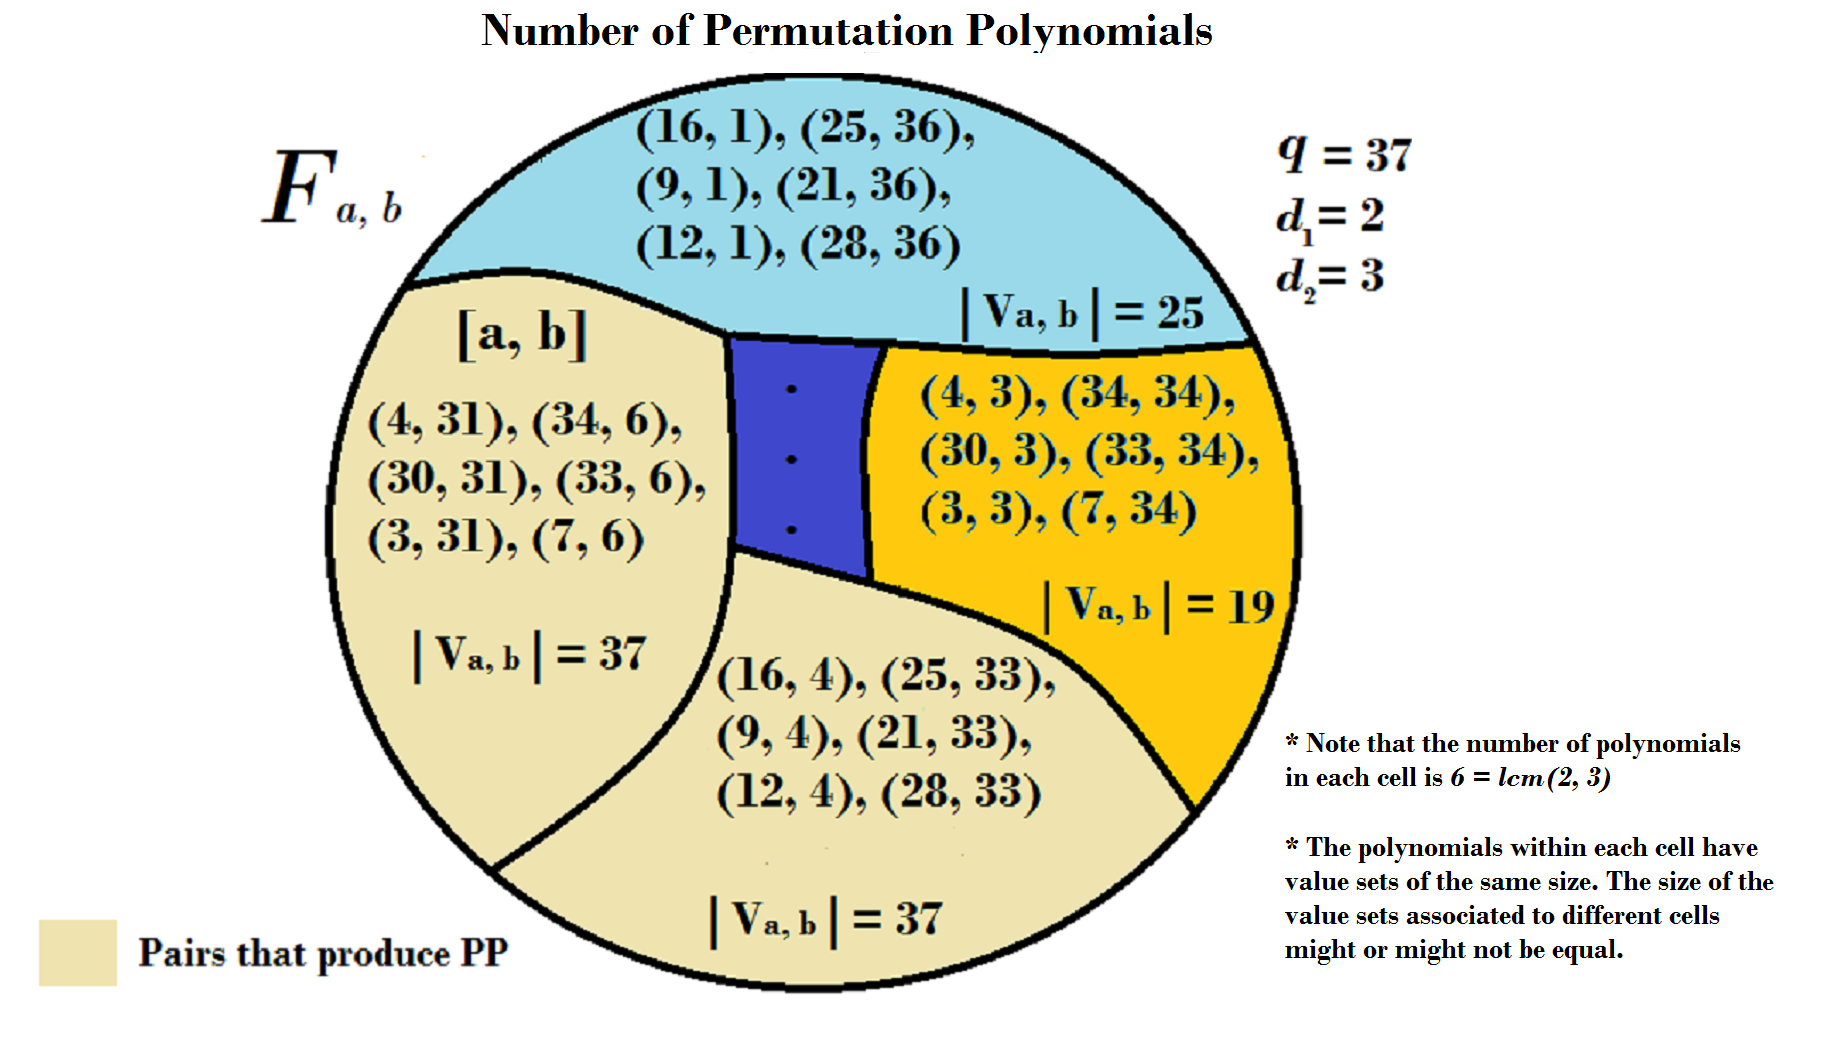
\includegraphics[width=11cm, height=6cm]{clases}
\end{frame}

\begin{frame}{Value set correspondence}

  {\Large $$f_{a,b}(X) = X^r(X^{\frac{q-1}{d_1}} + aX^{\frac{q-1}{d_2}} +b)$$}

  $$$$

  \begin{theorem}

    Suppose that $f_{a, b} \sim f_{a',b'}$ then $|V(f_{a, b})| = |V(f_{a', b'})|$.

  \end{theorem}

  \begin{example}
    Let $q = 13, d_1 = 2, d_2 = 3, a = 4, b = 8$. Since $(2^2,2^3) \sim (2^4,2^9)$ we have that $|V(f_{2^2, 2^3})| = |V(f_{2^4, 2^9})|$
  \end{example}

\end{frame}

\begin{frame}{Size of equivalence classes}
  
  {\Large $$f_{a,b}(X) = X^r(X^{\frac{q-1}{d_1}} + aX^{\frac{q-1}{d_2}} +b)$$}

  $$$$

  \begin{proposition}
    $|[f_{a, b}]| = lcm(d_1,d_2)$ where $lcm(x,y)$ is the least common multiple of $x$ and $y$.
  \end{proposition}

  \begin{example}
    Let $q = 13, d_1 = 2, d_2 = 3, a = 4, b = 8$. Note that $lcm(2,3) = 6$ These are the elements of $(a,b)$:
    $$ (2^2, 2^3), (2^4, 2^9), (2^6, 2^3), (2^8, 2^9), (2^10, 2^3), (2^{12}, 2^9), (2^2, 2^3) $$
  \end{example}
\end{frame}

\begin{frame}{Polynomials Results}
  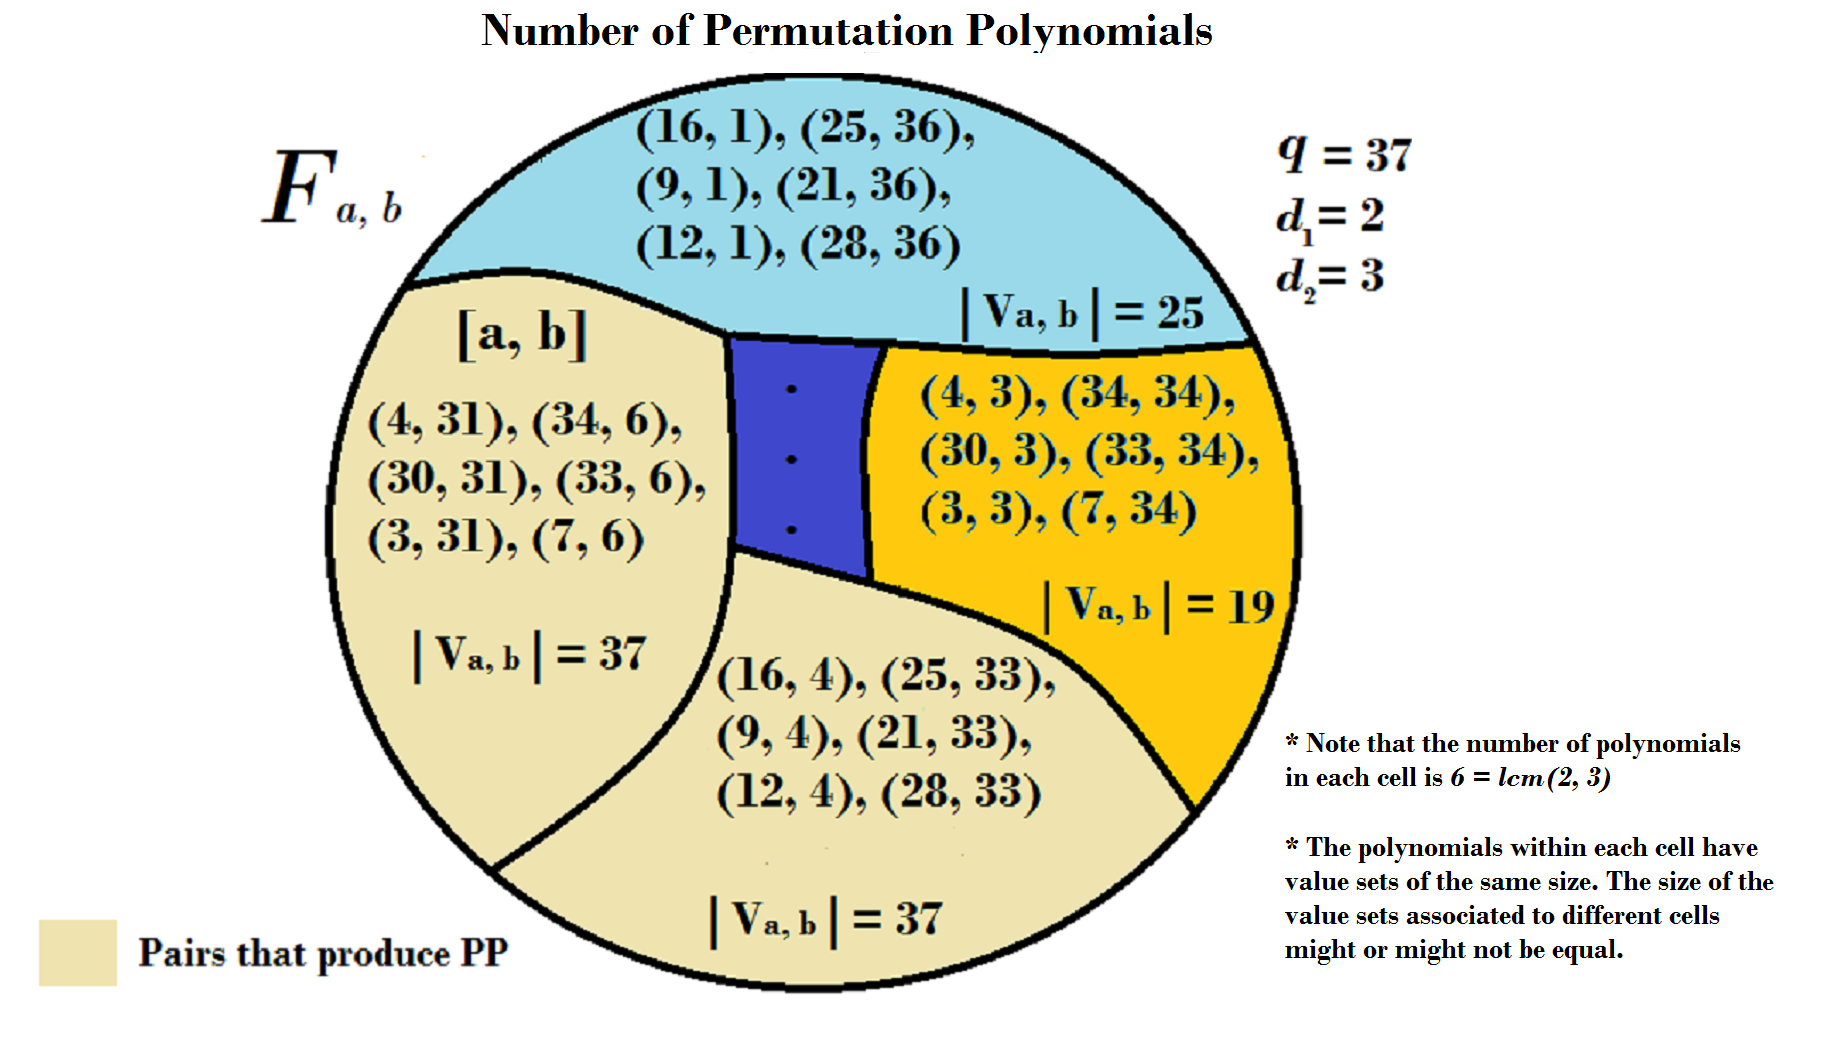
\includegraphics[width=11cm, height=6cm]{clases}
\end{frame}

\begin{frame}{Polynomial Results}
    \begin{proposition}
    The number of polynomials of the form $f_{a, b}(X)$ with $|V(f_{a, b})| = n$ is a multiple of $lcm(d_1, d_2)$
  \end{proposition}

  \begin{corollary}
    The number of permutation polynomials of the form $f_{a, b}(X)$ is a multiple of $lcm(d_1, d_2)$
  \end{corollary}
\end{frame}

% subsection families_of_polynomials_with_same_size_value_sets (end)

% \subsection{Construction of families of permutation trinomials} % (fold)
% \label{sub:construction_of_families_of_permutation_trinomials}

% \begin{frame}\frametitle{Constructing permutation trinomials}
    
% The following proposition gives us sufficient conditions for $f_{a,b}$ to be a permutation polynomial.

% \begin{proposition}
%   Suppose that $d\mid q-1$, $a, b \in \mathbb{F}_{q}$, $gcd(r, \frac{q^m-1}{r})=1$, and $h(X)=X^{\frac{d}{d_1}}+aX^{\frac{d}{d_2}}+b$. Let $gara = \alpha^{\frac{q-1}{d}}$, where $\alpha$ is a primitive root in $\mathbb{F}_{q}$. If $ (h(gara^i)/h(gara^j))^{\frac{q-1}{d}}=1 $ for all $0\leq i < j < d$, then $f_{a,b}(X)$ is a permutation polynomial of $\mathbb{F}_{q}$. 
% \end{proposition}

% \end{frame}

% subsection construction_of_families_of_permutation_trinomials (end)

\begin{frame}{Future Work}
  \begin{itemize}
    \item Find necessary and sufficient conditions such that $V(f_{a,b}) = \mathbb{F}_q$
    \item Collect data on number of permutation polynomials of the form $f_{a,b}$ for different values of $d_1$ and $d_2$ and compare results with number of permutation polynomials.
  \end{itemize}
\end{frame}

% section results (end)


\end{document}


